\documentclass{article}
\usepackage{tikz}
\usepackage{amsmath}
\usepackage{tabto}
\usepackage{fancyhdr}
\usepackage[margin=0.5in]{geometry}
\usetikzlibrary{arrows}
\begin{document}
\huge
Ejercicio \# 2
\begin{center}
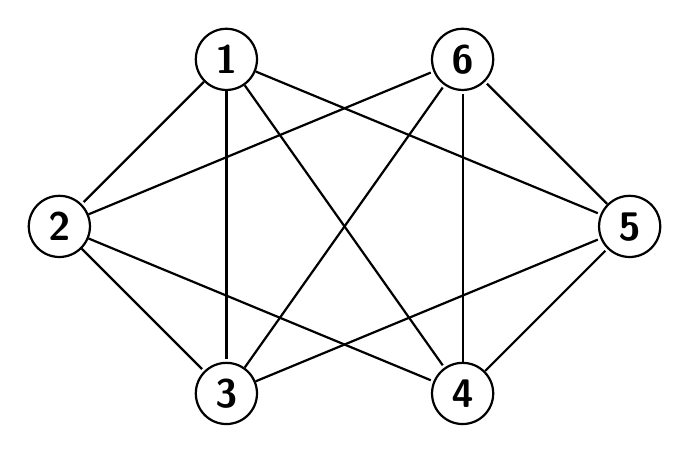
\begin{tikzpicture}[>=stealth',shorten >=1pt,auto,node distance=3cm,
                    thick,main node/.style={circle,draw,font=\sffamily\Large\bfseries}]

  \node[main node] (1) {1};
  \node[main node] (2) [below left of=1] {2};
  \node[main node] (3) [below right of=2] {3};
  \node[main node] (4) [right of=3] {4};
  \node[main node] (5) [above right of=4] {5};
  \node[main node] (6) [right of=1] {6};

  \path[every node/.style={font=\sffamily\small}]
    (1) edge node [left] {} (5)
		edge node [left] {} (4)
		edge node [left] {} (3)
		edge node [left] {} (2)
    (2) edge node [left] {} (3)
    	edge node [left] {} (4)
    	edge node [left] {} (6)
    (3) edge node [left] {} (5)
    	edge node [left] {} (6)
    (4)	edge node [left] {} (5)
    	edge node [left] {} (6)
    (5)	edge node [left] {} (6);
\end{tikzpicture}

\Large
$Nodos = {1,2,3,4,5,6}$ \\
\[
Vertices = \begin{bmatrix}
    \langle 1,2 \rangle & \langle 1,3 \rangle & \langle 1,4 \rangle & \langle 1,5 \rangle \\
    \langle 2,3 \rangle & \langle 2,4 \rangle & \langle 2,6 \rangle & \langle 3,5 \rangle \\
    \langle 3,6 \rangle & \langle 4,5 \rangle & \langle 4,6 \rangle & \langle 5,6 \rangle \\
\end{bmatrix}
\]
\end{center}
\huge
Ejercicio \# 3\\
\Large

a. La estrucutra que puede simular la tirada de un dado es una estructura de caminos, trayectos que pasan por diferentes \emph{Nodos}, a travez de los vertices.\\

b. Para generar la estructura de caminos se puede utilizar el siguiente algoritmo:\\
\hspace*{1cm} 1. Inicio\\ 
\hspace*{1cm} 2. Generar un numero aleatorio entre 1 y 10 (Esto decidira la cantidad de pasos \hspace*{2cm}que el dado dará a travez de los caminos)\\
\hspace*{1cm} 3. Si \emph{i} (un contador) es menor o igual al numero de pasos, entonces seguir al paso \hspace*{2cm}4, de lo contrario avanzar al paso 8\\
\hspace*{1cm} 4. Generar un numero de 1 a 4\\
\hspace*{1cm} 5. Avanzar por el vertice numerado con el numero generado en el paso 4.\\
\hspace*{1cm} 6. sumar una unidad al contador \emph{i}.\\
\hspace*{1cm} 7. regresar al paso 3\\
\hspace*{1cm} 8. Fin\\

c. El algorito asegura un resultado ya que utiliza un contador con una condicional, lo \hspace*{1cm}cual asegura que la simulación del dado genera un resultad\\
\\
\\
\large
Jose Mario Yon Cordon
\end{document}